% MLA golden: what is special about Multi-head Latent Attention (DeepSeek-V2/V3).
% Adapted by hand from tensor_dsl/examples/tikz/mla.tex. Standard attention is one block;
% the low-rank Q and KV paths, the decoupled RoPE branch and the KV cache (c^KV + k^R) are drawn out.
% Build: pdflatex mla.tex && pdftoppm -png -r 220 -singlefile mla.pdf mla
\documentclass[border=10pt]{standalone}
\usepackage{amsmath,amssymb}
\usepackage{tikz}
\usetikzlibrary{arrows.meta,backgrounds,calc,fit,positioning}

\definecolor{paperpink}{HTML}{F4DADA}
\definecolor{paperlavender}{HTML}{E9E4F1}
\definecolor{papergreen}{HTML}{DDECDD}
\definecolor{paperblue}{HTML}{E2ECF4}
\definecolor{cachefill}{HTML}{FFF6DA}
\definecolor{cacheink}{HTML}{B8860B}
\definecolor{ink}{HTML}{252525}
\definecolor{muted}{HTML}{57606A}

\begin{document}
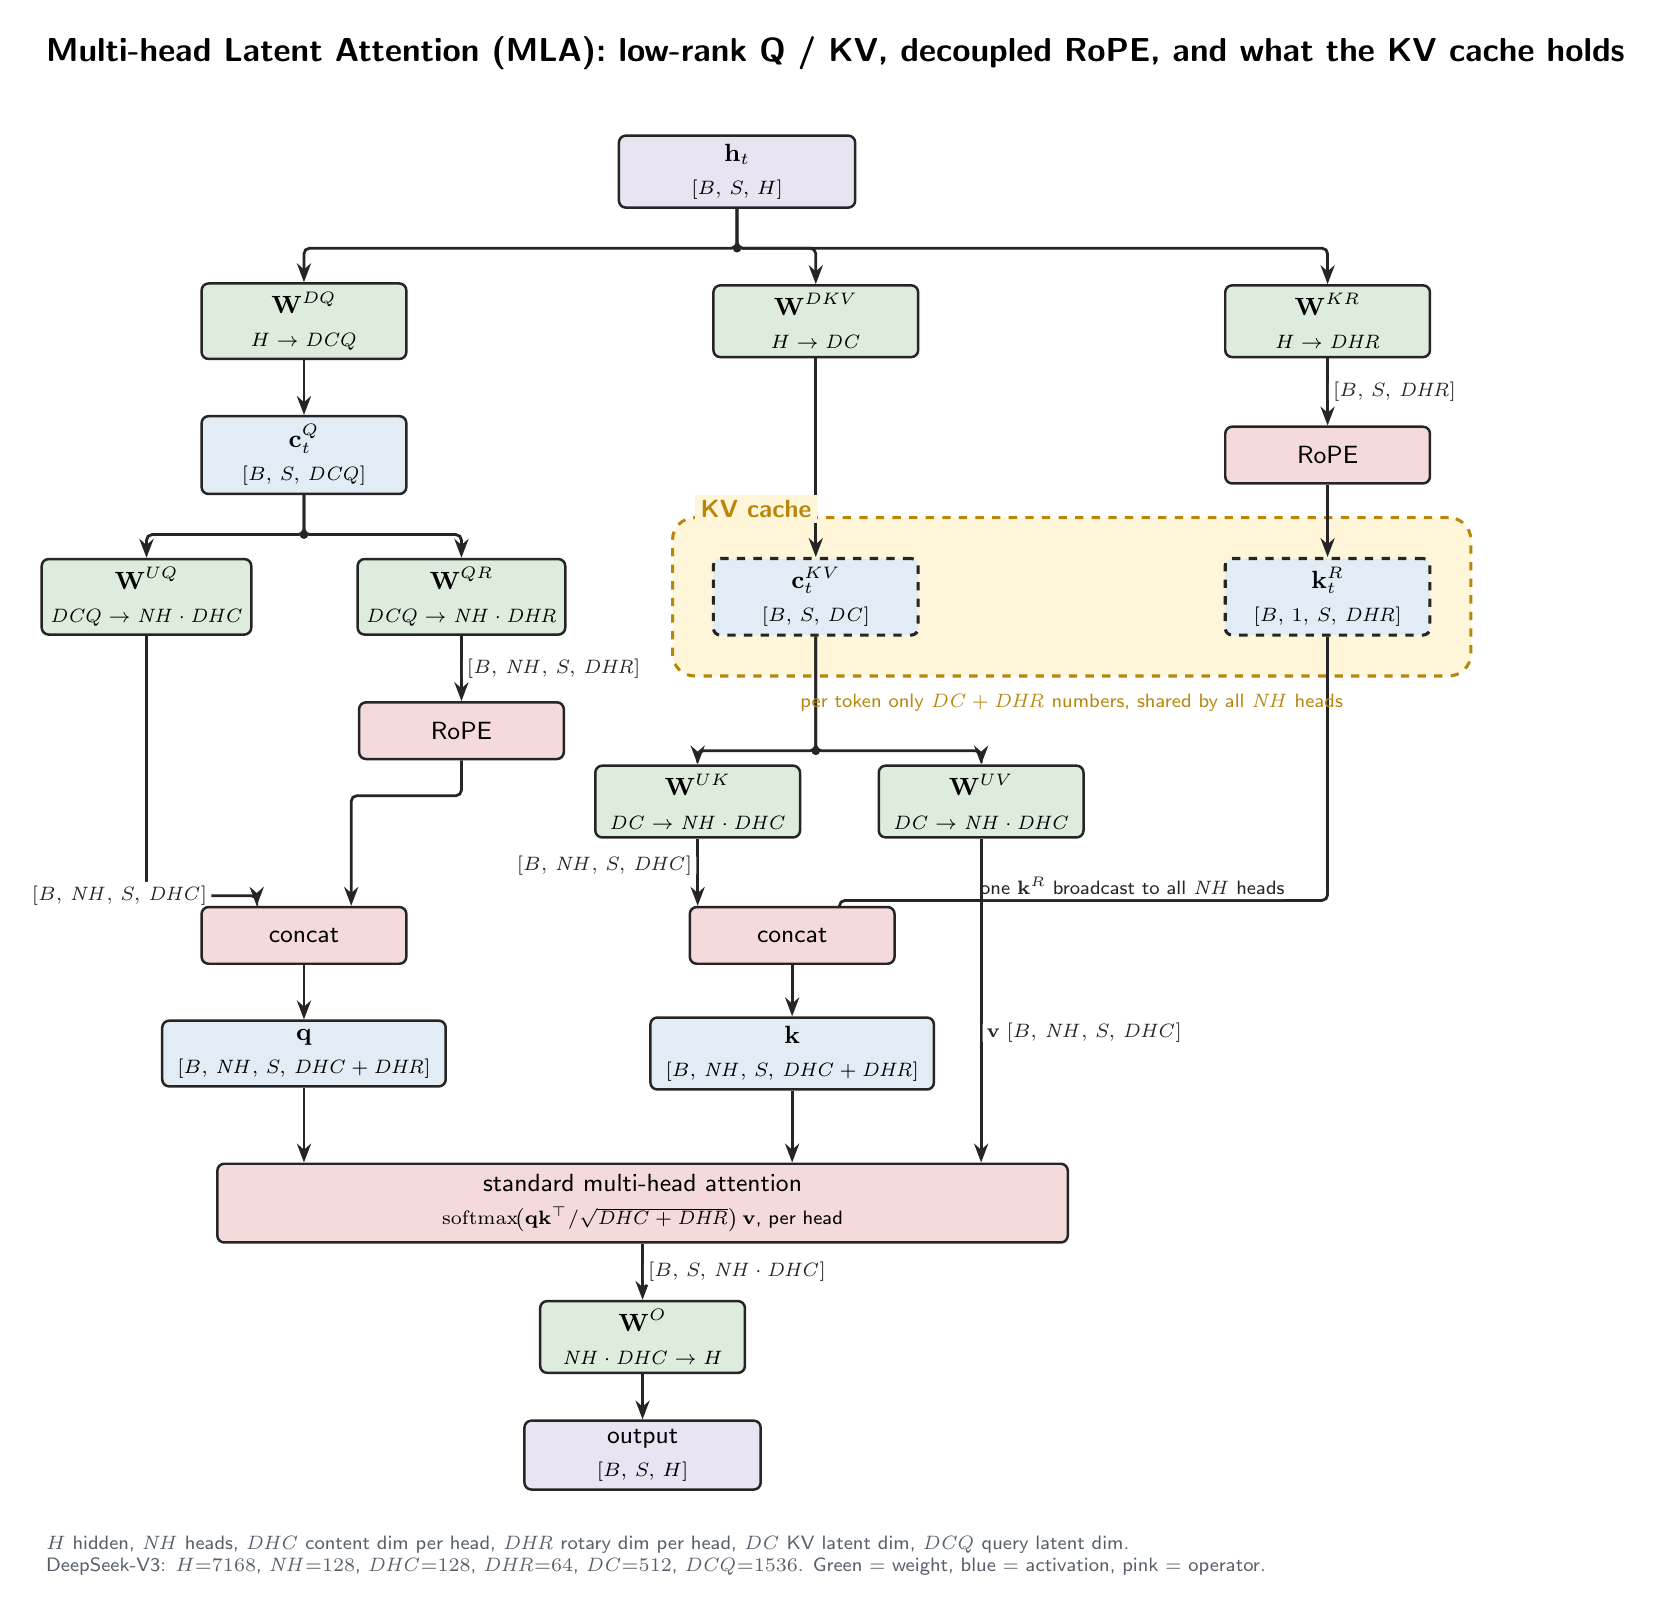
\begin{tikzpicture}[
  >={Stealth[length=2.4mm]},
  font=\sffamily\small,
  io/.style={draw=ink,fill=paperlavender,rounded corners=2.5pt,line width=.9pt,minimum width=3.0cm,minimum height=0.8cm,align=center,inner sep=3pt},
  op/.style={draw=ink,fill=paperpink,rounded corners=2.5pt,line width=.9pt,minimum width=2.6cm,minimum height=0.72cm,align=center,inner sep=3pt},
  weight/.style={draw=ink,fill=papergreen,rounded corners=2.5pt,line width=.9pt,minimum width=2.6cm,minimum height=0.8cm,align=center,inner sep=3pt},
  act/.style={draw=ink,fill=paperblue,rounded corners=2.5pt,line width=.9pt,minimum width=2.6cm,minimum height=0.8cm,align=center,inner sep=3pt},
  cached/.style={act,dashed,line width=1.1pt},
  flow/.style={draw=ink,line width=1.0pt,->,rounded corners=2pt},
  dimlabel/.style={font=\sffamily\scriptsize,text=ink,fill=white,inner sep=1.5pt},
  note/.style={font=\sffamily\scriptsize,text=muted,align=left},
  title/.style={font=\sffamily\bfseries\large,anchor=west},
]
  % ── input and down-projections ────────────────────────────────────────────
  \node[io] (h) at (0.5,0) {$\mathbf{h}_t$\\[1pt]{\scriptsize $[B,\,S,\,H]$}};
  \node[weight] (wdq)  at (-5,-1.9) {$\mathbf{W}^{DQ}$\\[1pt]{\scriptsize $H \to \mathit{DCQ}$}};
  \node[weight] (wdkv) at (1.5,-1.9) {$\mathbf{W}^{DKV}$\\[1pt]{\scriptsize $H \to \mathit{DC}$}};
  \node[weight] (wkr)  at (8,-1.9) {$\mathbf{W}^{KR}$\\[1pt]{\scriptsize $H \to \mathit{DHR}$}};

  % ── query path: compress, then expand per head ────────────────────────────
  \node[act] (cq) at (-5,-3.6) {$\mathbf{c}^{Q}_t$\\[1pt]{\scriptsize $[B,\,S,\,\mathit{DCQ}]$}};
  \node[weight] (wuq) at (-7,-5.4) {$\mathbf{W}^{UQ}$\\[1pt]{\scriptsize $\mathit{DCQ} \to \mathit{NH}\cdot\mathit{DHC}$}};
  \node[weight] (wqr) at (-3,-5.4) {$\mathbf{W}^{QR}$\\[1pt]{\scriptsize $\mathit{DCQ} \to \mathit{NH}\cdot\mathit{DHR}$}};
  \node[op] (ropeq) at (-3,-7.1) {RoPE};

  % ── KV path and the decoupled RoPE key: the only per-token state that is cached ──
  \node[op] (ropek) at (8,-3.6) {RoPE};
  \node[cached] (ckv) at (1.5,-5.4) {$\mathbf{c}^{KV}_t$\\[1pt]{\scriptsize $[B,\,S,\,\mathit{DC}]$}};
  \node[cached] (kr)  at (8,-5.4) {$\mathbf{k}^{R}_t$\\[1pt]{\scriptsize $[B,\,1,\,S,\,\mathit{DHR}]$}};
  \node[weight] (wuk) at (0,-8.0) {$\mathbf{W}^{UK}$\\[1pt]{\scriptsize $\mathit{DC} \to \mathit{NH}\cdot\mathit{DHC}$}};
  \node[weight] (wuv) at (3.6,-8.0) {$\mathbf{W}^{UV}$\\[1pt]{\scriptsize $\mathit{DC} \to \mathit{NH}\cdot\mathit{DHC}$}};

  % ── per-head q and k: content part + rotary part ──────────────────────────
  \node[op] (qcat) at (-5,-9.7) {concat};
  \node[op] (kcat) at (1.2,-9.7) {concat};
  \node[act,minimum width=3.6cm] (q) at (-5,-11.2) {$\mathbf{q}$\\[1pt]{\scriptsize $[B,\,\mathit{NH},\,S,\,\mathit{DHC}+\mathit{DHR}]$}};
  \node[act,minimum width=3.6cm] (k) at (1.2,-11.2) {$\mathbf{k}$\\[1pt]{\scriptsize $[B,\,\mathit{NH},\,S,\,\mathit{DHC}+\mathit{DHR}]$}};

  % ── standard attention, collapsed ─────────────────────────────────────────
  \node[op,minimum width=10.8cm,minimum height=1.0cm] (attn) at (-0.7,-13.1)
    {standard multi-head attention\\[1pt]{\scriptsize $\mathrm{softmax}\!\big(\mathbf{q}\mathbf{k}^{\top}/\sqrt{\mathit{DHC}+\mathit{DHR}}\big)\,\mathbf{v}$, per head}};
  \node[weight] (wo) at (-0.7,-14.8) {$\mathbf{W}^{O}$\\[1pt]{\scriptsize $\mathit{NH}\cdot\mathit{DHC} \to H$}};
  \node[io] (out) at (-0.7,-16.3) {output\\[1pt]{\scriptsize $[B,\,S,\,H]$}};

  % ── KV cache: drawn as a boundary around exactly what is stored ────────────
  \begin{scope}[on background layer]
    \node[draw=cacheink,fill=cachefill,dashed,rounded corners=8pt,line width=1.1pt,inner sep=5mm,fit=(ckv)(kr)] (cache) {};
  \end{scope}
  \node[font=\sffamily\bfseries\small,text=cacheink,anchor=south west,fill=cachefill,inner sep=2pt] at ([xshift=3mm,yshift=-1mm]cache.north west) {KV cache};
  \node[note,text=cacheink,anchor=north] at ([yshift=-0.9mm]cache.south) {per token only $\mathit{DC}+\mathit{DHR}$ numbers, shared by all $\mathit{NH}$ heads};

  \begin{scope}[on background layer]
    \draw[flow] (h.south) -- ++(0,-0.5) -| (wdq.north);
    \draw[flow] (h.south) -- ++(0,-0.5) -| (wdkv.north);
    \draw[flow] (h.south) -- ++(0,-0.5) -| (wkr.north);
    \fill[ink] ([yshift=-0.5cm]h.south) circle[radius=0.055];

    \draw[flow] (wdq.south) -- (cq.north);
    \draw[flow] (cq.south) -- ++(0,-0.5) -| (wuq.north);
    \draw[flow] (cq.south) -- ++(0,-0.5) -| (wqr.north);
    \fill[ink] ([yshift=-0.5cm]cq.south) circle[radius=0.055];
    \draw[flow] (wqr.south) -- node[dimlabel,right] {$[B,\,\mathit{NH},\,S,\,\mathit{DHR}]$} (ropeq.north);
    \draw[flow] (wuq.south) -- ++(0,-3.3) -| node[dimlabel,pos=0.3,left] {$[B,\,\mathit{NH},\,S,\,\mathit{DHC}]$} ([xshift=-0.6cm]qcat.north);
    \draw[flow] (ropeq.south) -- ++(0,-0.45) -| ([xshift=0.6cm]qcat.north);

    \draw[flow] (wdkv.south) -- (ckv.north);
    \draw[flow] (wkr.south) -- node[dimlabel,right] {$[B,\,S,\,\mathit{DHR}]$} (ropek.north);
    \draw[flow] (ropek.south) -- (kr.north);
    \draw[flow] (ckv.south) -- ++(0,-1.45) -| (wuk.north);
    \draw[flow] (ckv.south) -- ++(0,-1.45) -| (wuv.north);
    \fill[ink] ([yshift=-1.45cm]ckv.south) circle[radius=0.055];
    \draw[flow] (wuk.south) -- node[dimlabel,left,pos=0.4] {$[B,\,\mathit{NH},\,S,\,\mathit{DHC}]$} ([xshift=-1.2cm]kcat.north);
    \draw[flow] (kr.south) -- ++(0,-3.35) -| node[dimlabel,pos=0.2,above] {one $\mathbf{k}^R$ broadcast to all $\mathit{NH}$ heads} ([xshift=0.6cm]kcat.north);

    \draw[flow] (qcat.south) -- (q.north);
    \draw[flow] (kcat.south) -- (k.north);
    \draw[flow] (q.south) -- (q.south |- attn.north);
    \draw[flow] (k.south) -- (k.south |- attn.north);
    \draw[flow] (wuv.south) -- node[dimlabel,right,pos=0.6] {$\mathbf{v}\;[B,\,\mathit{NH},\,S,\,\mathit{DHC}]$} (wuv.south |- attn.north);
    \draw[flow] (attn.south) -- node[dimlabel,right] {$[B,\,S,\,\mathit{NH}\cdot\mathit{DHC}]$} (wo.north);
    \draw[flow] (wo.south) -- (out.north);
  \end{scope}

  % ── title and symbols ─────────────────────────────────────────────────────
  \node[title] at (-8.4,1.5) {Multi-head Latent Attention (MLA): low-rank Q / KV, decoupled RoPE, and what the KV cache holds};
  \node[note,anchor=north west] at (-8.4,-17.2) {$H$ hidden, $\mathit{NH}$ heads, $\mathit{DHC}$ content dim per head, $\mathit{DHR}$ rotary dim per head, $\mathit{DC}$ KV latent dim, $\mathit{DCQ}$ query latent dim.\\
    DeepSeek-V3: $H{=}7168$, $\mathit{NH}{=}128$, $\mathit{DHC}{=}128$, $\mathit{DHR}{=}64$, $\mathit{DC}{=}512$, $\mathit{DCQ}{=}1536$. Green = weight, blue = activation, pink = operator.};
\end{tikzpicture}
\end{document}
